%!TEX program = Xelatex
\documentclass{article}
\usepackage{amsmath,amscd,amsbsy,amssymb,latexsym,url,bm,amsthm}
\usepackage{epsfig,graphicx,subfigure}
\usepackage{enumitem,balance,mathtools}
\usepackage{wrapfig}
\usepackage{mathrsfs, euscript}
\usepackage{hyperref}
\usepackage{listings}
\usepackage[ruled,lined,boxed,linesnumbered]{algorithm2e}
\usepackage{algorithmic}
\usepackage[UTF8]{ctex}
\usepackage{setspace}
\usepackage{color,xcolor}
\newtheorem{theorem}{Theorem}[section]
\newtheorem{lemma}[theorem]{Lemma}
\newtheorem{proposition}[theorem]{Proposition}
\newtheorem{corollary}[theorem]{Corollary}
\newtheorem{exercise}{Exercise}[section]
\newtheorem*{solution}{Solution}

\renewcommand{\thefootnote}{\fnsymbol{footnote}}
\newcommand{\postscript}[2]
{\setlength{\epsfxsize}{#2\hsize}
	\centerline{\epsfbox{#1}}}
\renewcommand{\baselinestretch}{1.0}

\setlength{\oddsidemargin}{-0.365in}
\setlength{\evensidemargin}{-0.365in}
\setlength{\topmargin}{-0.3in}
\setlength{\headheight}{0in}
\setlength{\headsep}{0in}
\setlength{\textheight}{10.1in}
\setlength{\textwidth}{7in}

% ------ adjust it according to the specific circumstances ----- %
\title{Project 1: CUDA实现的二维卷积}
\author{杨晨宇}
\date{517030910386}
% ---------------------------------------------------------------%
\definecolor{mygreen}{rgb}{0,0.6,0}
\lstset{
	numbers=left,                        % 设置行号
	columns=fullflexible,
	breaklines=true,                 % automatic line breaking only at whitespace
	captionpos=b,                    % sets the caption-position to bottom
	tabsize=4,                       % 把tab扩展为4个空格,默认是8个太长
	keywordstyle=\color{blue},
	commentstyle=\color{mygreen},    % 设置注释颜色	escapeinside={\%*}{*)},          % if you want to add LaTeX within your code
	frame=single,                        % 设置有边框
	language=C++,
}

\begin{document}
\maketitle

\section{要求}
本次实验中,我们将要利用CUDA编程实现深度学习中二维卷积的功能。

卷积计算包括两个输入: 特征图和卷积核。特征图是四维的张量[N, C, H, W],卷积核的尺寸[F, C, K, K]。二维卷积的概念在这里不再赘述。本次实验中,我们不考虑如stride等其他参数,因此输出的四维张量形状应为[N, F, H-K+1, W-K+1], 我们将它记作[N, F, H\_, W\_]。

为了进一步简化问题,我们假设特征图的尺寸是[8, 64, 128, 128],卷积核大小[128, 64, 3, 3],所有数据都为浮点数类型。我们需要先实现一个CPU版本的卷积,再将移植到GPU上(问题1);进一步地,我们需要对问题1中得到的程序进行优化,使它能够获得更高的计算效率(问题2)。


\section{背景介绍}
CUDA编程模型是一个异构模型,需要CPU和GPU协同工作。在CUDA中,host和device是两个重要的概念,我们用host指代CPU及其内存,而用device指代GPU及其内存。CUDA程序中既包含host程序,又包含device程序,它们分别在CPU和GPU上运行。同时,host与device之间可以进行通信,这样它们之间可以进行数据拷贝。典型的CUDA程序的执行流程如下:
\begin{enumerate}
	\item 分配host内存,并进行数据初始化;
	\item 分配device内存,并从host将数据拷贝到device上;
	\item 调用CUDA的核函数在device上完成指定的运算;
	\item 将device上的运算结果拷贝到host上;
	\item 释放device和host上分配的内存。
\end{enumerate}
\begin{figure}[h]
	\centering
	\includegraphics[width=0.7\linewidth]{1.jpg}
	\caption{GPU基本结构}
	\label{fig:gpu}
\end{figure}


\section{项目实现}
\subsection{CPU版本}
CPU版本的程序主要用来和后续实验进行对照,通过7个嵌套的循环依次计算输出张量的每个坐标点,虽然理解上比较直观,但单线程的计算方式使得它效率极低。
\begin{lstlisting}
void Conv2D_cpu(Matrix &out, Matrix fm, Matrix kn) {
	out.fill_value(0);
	for (int bsize = 0; bsize < fm.d1; bsize++)
		for (int f = 0; f < kn.d1; f++)
			for (int c = 0; c < kn.d2; c++)
				for (int h_ = 0; h_ < fm.d3 - kn.d3 + 1; h_++)
					for (int w_ = 0; w_ < fm.d4 - kn.d4 + 1; w_++)
						for (int i = 0; i < kn.d3; i++)
							for (int j = 0; j < kn.d4; j++)
								*out.get(bsize, f, h_, w_) += 
								   *kn.get(f, c, i, j) * *fm.get(bsize, c, h_+i, w_+j);
} 
\end{lstlisting}

\subsection{单线程的CUDA实现}
想要利用CUDA来进行计算,首先要在device(GPU)上分配内存,并将数据从host(CPU)迁移到GPU上,这里需要用到\textit{cudaMalloc()}和\textit{cudaMemcpy()}函数,前者在GPU中分配一块内存,后者则实现数据的迁移。要释放分配的内存,则使用\textit{cudaFree()}函数。这里我将内存的迁移与分配/释放都写在了Matrix类内置函数中。

原本该部分实验仅要求将之前的CPU版本的程序移植到CPU上,对性能暂不考虑。但由于GPU线程并行且轻量级的特性,单线程的计算会比CPU更加缓慢(实验结果也确实如此)。经过权衡,我将数据根据batch进行划分,每个样本对应一个线程块,每个线程块中仍然是单线程进行计算。对应到核函数中,则是去掉了最外层的循环,其他部分与CPU版本保持一致。

\begin{lstlisting}
void Conv2D_cuda(Matrix &out, Matrix fm, Matrix kn) {
	fm.cuda(); kn.cuda(); out.cuda();
	// divide by sample, each sample has a single thread;
	conv2d_cuda_kernel<<<fm.d1,1>>>(out.element, fm.element, kn.element, 
										kn.d2, kn.d1, fm.d3, fm.d4, kn.d3, kn.d4);
	out.cpu();
}

__global__ void conv2d_cuda_kernel(float *out_matr, float *fm_matr, float *kn_matr,
									int in_channel, int out_channel, int height, int width, 
									int ksize_x, int ksize_y) {
	int batch_id = blockIdx.x;
	for (int channel_id = 0; channel_id < out_channel; channel_id++)
		for (int row = 0; row < height - ksize_x + 1; row++)
			for (int col = 0; col < width - ksize_y + 1; col++) { \\ each position of the output tensor
				float cell_value = 0;
				for (int c = 0; c < in_channel; c++) // each in-channel
					for (int i = 0; i < ksize_x; i++) 
						for (int j = 0; j < ksize_y; j++) // each location of a kernel 
							cell_value += kn_matr[channel_id*in_channel*ksize_x*ksize_y + c*ksize_x*ksize_y + i*ksize_y + j] * fm_matr[batch_id*in_channel*height*width + c*height*width + (row+i)*width + (col+j)];
							
				out_matr[batch_id*out_channel*(height - ksize_x + 1)*(width - ksize_y + 1) + channel_id*(height - ksize_x + 1)*(width - ksize_y + 1) + row*(width - ksize_y + 1) + col] = cell_value;
			}
}
\end{lstlisting}
\subsection{CUDA优化}
对比前两段程序的结果(见第4节)不难看出,仅仅是划分为八个线程块,原程序计算时间已经缩减了一半多——而事实上,对于大小为[8, 128, 126, 126]的输出张量而言,其每一个点的计算过程相对于其他点都是独立的,因此我们最多可以将其分为 $(8\times128\times126\times126)$ 个子线程,每个子线程分别计算单个卷积核对于特征图上某个位置的卷积,即两个[64, 3, 3]的张量的点乘。

考虑到每个线程块中的线程数是有上限的(一般为1024),因此在具体实现过程中,我们设置线程块数目为$(126\times126)$,使得每个线程块内部刚好包含$(8\times128)$个线程,从而充分利用GPU资源。在核函数中,我们通过\textit{blockIdx}和\textit{threadIdx}唯一确定该线程对应特征图上的位置及所使用的卷积核。
\begin{lstlisting}
void Conv2D_cuda_optim(Matrix &out, Matrix fm, Matrix kn) {
	fm.cuda(); kn.cuda(); out.cuda();
	dim3 block_sz(out.d1, out.d2); // batch_size * out_channel
	dim3 grid_sz(out.d3, out.d4); // height * weight
	conv2d_cuda_optim_kernel<<<grid_sz,block_sz>>>(out.element, fm.element, kn.element, 
	kn.d2, kn.d1, fm.d3, fm.d4, kn.d3, kn.d4);
	out.cpu();
}

__global__ void conv2d_cuda_optim_kernel(float *out_matr, float *fm_matr, float *kn_matr,
				int in_channel, int out_channel, int height, int width, 
				int ksize_x, int ksize_y) {
	int batch_id = threadIdx.x, channel_id = threadIdx.y;
	int row = blockIdx.x, col = blockIdx.y;
	float cell_value = 0;
	for (int c = 0; c < in_channel; c++) // each in-channel
		for (int i = 0; i < ksize_x; i++) 
			for (int j = 0; j < ksize_y; j++) // each lacation of a kernel 
				cell_value += kn_matr[channel_id*in_channel*ksize_x*ksize_y + c*ksize_x*ksize_y + i*ksize_y + j] * fm_matr[batch_id*in_channel*height*width + c*height*width + (row+i)*width + (col+j)];

	out_matr[batch_id*out_channel*(height - ksize_x + 1)*(width - ksize_y + 1) + channel_id*(height - ksize_x + 1)*(width - ksize_y + 1) + row*(width - ksize_y + 1) + col] = cell_value;
}
\end{lstlisting}

\section{实验结果}
\begin{figure}[h]
	\centering
	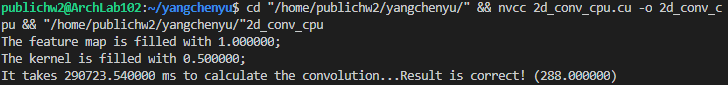
\includegraphics[width=1\linewidth]{result_cpu}
	\caption{CPU串行版本}
	\label{fig:cpu}
\end{figure}
\begin{figure}[h]
	\centering
	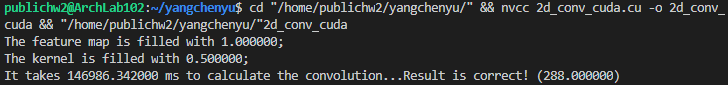
\includegraphics[width=1\linewidth]{result_cuda}
	\caption{未优化的GPU版本(8线程块)}
	\label{fig:gpu}
\end{figure}
\begin{figure}[h]
	\centering
	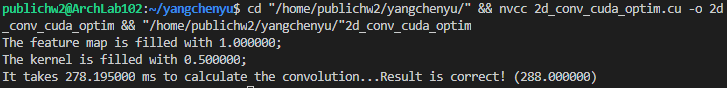
\includegraphics[width=1\linewidth]{result_cuda_optim}
	\caption{优化过后的GPU版本}
	\label{fig:gpu}
\end{figure}

	

\end{document}